\chapter{Anhang}
\section{Aufgabe 1}
\begin{figure}[H]
    \centering
    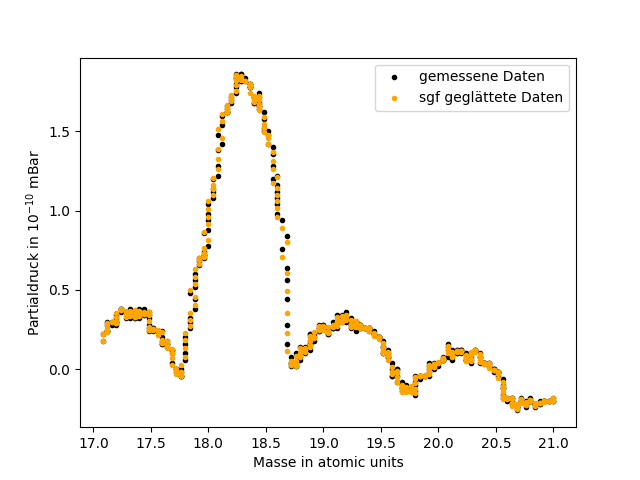
\includegraphics[width=140mm,scale=0.8]{Massenspektrometer/include/MSm18Wasser.png}
    \caption{Peak bei \SI{18}{amu}, Wasser}
    \label{fig:MSWasserPeak}
\end{figure}
\begin{figure}[H]
    \centering
    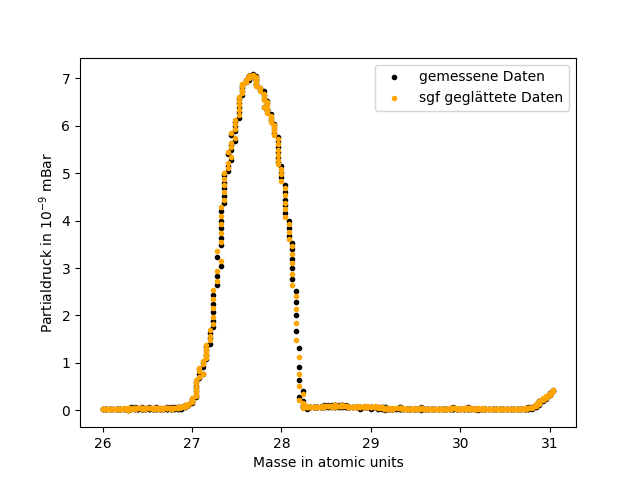
\includegraphics[width=140mm,scale=0.8]{Massenspektrometer/include/MSm28N2.png}
    \caption{Peak bei \SI{28}{amu}, molekularer Stickstoff}
    \label{fig:MSN2Peak}
\end{figure}
\begin{figure}[H]
    \centering
    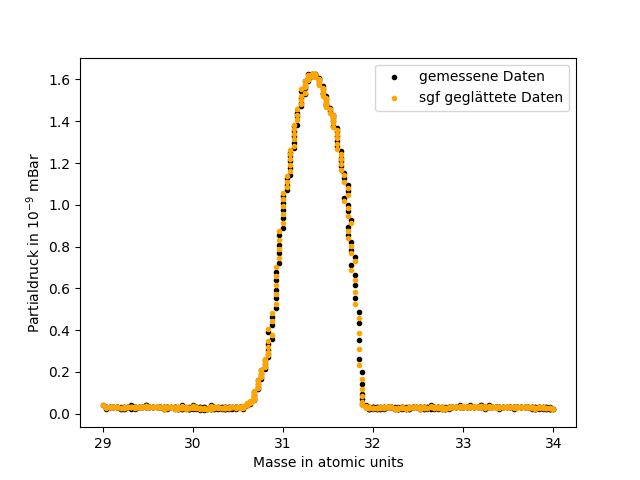
\includegraphics[width=140mm,scale=0.8]{Massenspektrometer/include/MSm32O2.png}
    \caption{Peak bei \SI{32}{amu}, molekularer Sauerstoff}
    \label{fig:MSO2Peak}
\end{figure}
\begin{figure}[H]
    \centering
    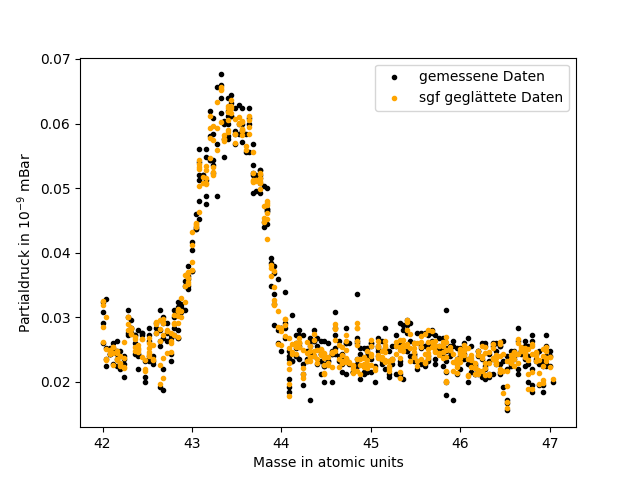
\includegraphics[width=140mm,scale=0.8]{Massenspektrometer/include/MSm44CO2.png}
    \caption{Peak bei \SI{44}{amu}, Kohlendioxid}
    \label{fig:MSCO2Peak}
\end{figure}
\section{Aufgabe 5}
\begin{figure}[H]
    \centering
    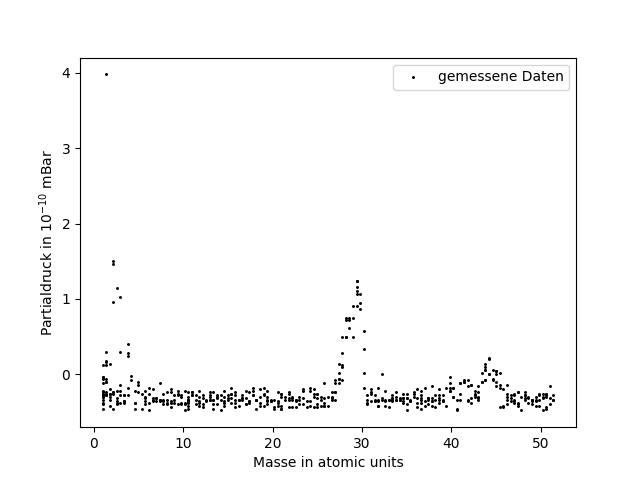
\includegraphics[width=120mm,scale=0.8]{Massenspektrometer/include/MS30eV.png}
    \caption{Spektrum des unbekannten Gases bei einer Elektronenenergie von \SI{30}{eV}}
    \label{fig:MS30eV}
\end{figure}

\begin{figure}[H]
    \centering
    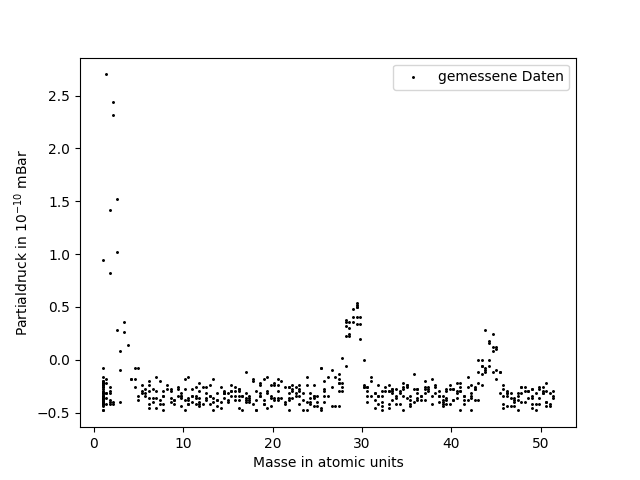
\includegraphics[width=120mm,scale=0.8]{Massenspektrometer/include/MS20eV.png}
    \caption{Spektrum des unbekannten Gases bei einer Elektronenenergie von \SI{20}{eV}}
    \label{fig:MS20eV}
\end{figure}
